\section{Design-Space Ablations, Related Preconditioners, and Mechanism}
\label{sec:analysis}

Having established \emph{that} \mname{WT-MLP-Lag} improves fixed-token pretraining across seeds, horizons, and widths, we now answer \emph{why} each component of its design is necessary:
we ablate factor placement across all 19 taxonomic variants (\Cref{sec:ablations}), compare head-to-head against recent curvature-aware polar optimizers \mname{GO-MUON} and \mname{Mousse} (\Cref{sec:related_baselines}), verify via counterfactual direction grafting that output roots act by subspace rotation rather than step-size inflation (\Cref{sec:mechanism}), and map the multi-scale \texttt{130M} and \texttt{520M} quality--wall-clock Pareto frontiers (\Cref{sec:pareto}).

\subsection{Controlled Factor-Placement and Approximation Ablations}
\label{sec:ablations}

\Cref{tab:ablations} and \Cref{fig:ablations_related}a isolate five structural design questions on matched \texttt{130M} ($2.68\text{B}$-token, \texttt{seed 0}) trajectories:

\begin{enumerate}[leftmargin=1.6em, itemsep=2pt, topsep=2pt]
  \item \textbf{Output preconditioning is complementary to, never a substitute for, input whitening.}
  Replacing input factors with dense output factors everywhere (\mname{Abl-OutOnly}, mirror image of \mname{MuonT}) degrades late $\Lsel$ by $+0.0087$ nats---performing even worse than unpreconditioned \mname{Muon} ($+0.0055$)!
  Even swapping only $W_{\mathrm{down}}$'s $2{,}048$-wide input root for a $512$-wide output root (\mname{Abl-DownSwap}) loses $+0.0025$ nats.
  Similarly, diagonalizing \emph{both} sides (\mname{Abl-BothDiag}) loses $+0.0180$ nats because $\dm$-wide inputs carry $>98\%$ rotational anisotropy (\Cref{tab:diagnosis}).
  \item \textbf{Diagonalizing \texttt{gate,up} matches or slightly exceeds full dense outputs, whereas dropping them halves the gain.}
  Comparing \mname{WT-MLP} ($-0.0066$ late $\Lsel$) against full dense \mname{DT-All} ($-0.0058$) confirms that removing $\dff$-wide output rotations sacrifices \emph{zero} held-out quality---in fact edging slightly ahead because exact per-step diagonal scaling avoids 4-step cached-basis staleness on rapidly drifting \texttt{gate/up} moments while cutting rank-0 exact fallbacks by $39\%$ ($32{,}838 \to 19{,}998$).
  Conversely, omitting \texttt{gate/up} output factors altogether (\mname{Abl-No2048}) forfeits over half the gain ($-0.0031$ vs.\ $-0.0066$), proving that pre-SwiGLU coordinate scale carries genuine optimization signal.
  \item \textbf{Both inner ($-1/2$) and outer ($-1/8$) left factors contribute.}
  Applying dense left factors only \emph{outside} $\Nten$ (\mname{Abl-OuterDense}, $L=I$) drops late $\Lsel$ gain from $-0.0058$ to $-0.0040$ (and diagonal outer-only \mname{OD-Outer} drops from $-0.0029$ to $-0.0020$ in fixed-age Wave 7), demonstrating that pre-$\Nten$ singular-frame rotation accounts for roughly one-third of the benefit.
  \item \textbf{Asymmetric (\mname{WT-MLP-Lag}) vs.\ symmetric (\mname{WT-Sym-Lag}) $\dff$ thresholding.}
  What if we apply the exact same width rule symmetrically to the input side by also diagonalizing $\dff$-wide \texttt{in:down} (\mname{WT-Sym-Lag})?
  In a same-wave head-to-head run (\texttt{wave\_sym\_fastlag}), \mname{WT-Sym-Lag} cuts benchmark step overhead to just $+3.32\%$ ($20.82\text{ GiB}$ peak memory) and still beats \mname{MuonT} at completion ($-0.0025$ final $\Lsel$, $-0.0029$ final $\Lc$), \emph{but} lags \mname{WT-MLP-Lag} by $+0.0181 \pm 0.0024$ nats in the first $537\text{M}$-token training window and $+0.0036$ nats in late $\Lsel$.
  Why? Unlike pre-SwiGLU \texttt{out:gate,up} ($\rho_{\mathrm{rms}} = 0.0048\text{--}0.0082$, $77.9\%\text{--}90.8\%$ diagonal anisotropy), post-SwiGLU \texttt{in:down} retains $56.6\%\text{--}79.7\%$ off-diagonal moment anisotropy across \mname{Muon}, \mname{MuonT}, and \mname{WT-MLP-Lag} ($\rho_{\mathrm{rms}} = 0.0283 / 0.0346 / 0.0359$; \Cref{tab:diagnosis}) that substantially accelerates early-stage descent.
  \item \textbf{One-step asynchronous lag ($\tau = 1$) is nearly lossless.}
  Update-by-update paired differencing over the final $537\text{M}$ tokens shows \mname{WT-MLP-Lag} differs from synchronous \mname{WT-MLP} by just $+0.00011 \pm 0.00004$ nats in training loss ($+0.00033$ final $\Lsel$ in Wave 4; and \mname{DT-All-Lag} matches \mname{DT-All} to $-0.0001$ late $\Lsel$) while halving step-time overhead.
\end{enumerate}

\begin{table}[t]
  \centering
  \caption{\textbf{Controlled factor-placement and approximation ablations at \texttt{130M}} ($0.5\text{M}$ batch, $5{,}120$ steps, $2.68\text{B}$ tokens, \texttt{seed 0}, $\eta = 0.02263$ [$\eta=0.016$ for \mname{Muon}]). ``Late $\Delta\Lsel$'' and ``Late $\Delta\Lc$'' average the 11 second-half evaluations ($\text{steps } 2{,}751\text{--}5{,}120$) relative to \mname{MuonT}; ``$\Delta\mathcal{L}_{\mathrm{train}}$'' is the exact per-update paired training loss difference over the final $537\text{M}$ tokens ($\text{SE} \approx 0.00004\text{--}0.00016$); ``Bench $\Delta t$'' is the unified 8-GPU step-time overhead vs.\ \mname{MuonT} (\texttt{bench\_8gpu\_opt}).}
  \label{tab:ablations}
  \vspace{2pt}
  \resizebox{\textwidth}{!}{%
  \begin{tabular}{@{}llllrrrr@{}}
    \toprule
    Method & Right ($R,\hat{R}$) & Left ($L,\hat{L}$: $\dm \,/\, \dff$) & Special Setting & Late $\Delta\Lsel$ & Late $\Delta\Lc$ & $\Delta\mathcal{L}_{\mathrm{train}}$ & Bench $\Delta t$ \\
    \midrule
    \mname{Abl-BothDiag}   & Diag / Diag   & Diag / Diag   & Both sides diagonal & $+0.0180$ & $+0.0177$ & $+0.0134$ & $-0.4\%$ \\
    \mname{Abl-OutOnly}    & $I$ / $I$     & Dense / Dense & Drop all inputs     & $+0.0087$ & $+0.0109$ & $+0.0079$ & $+29.8\%$ \\
    \mname{Muon}           & $I$ / $I$     & $I$ / $I$     & $\eta = 0.016$      & $+0.0055$ & $+0.0053$ & $+0.0062$ & $-1.4\%$ \\
    \mname{Abl-DownSwap}   & $\text{down}\!=\!I$ & $\text{down}$ Dense & Swap \texttt{down} in$\to$out & $+0.0025$ & $+0.0036$ & $+0.0032$ & $+0.3\%$ \\
    \midrule
    \mname{MuonT}          & Dense / Dense & $I$ / $I$     & Reference baseline  & $0.0000$  & $0.0000$  & $0.0000$  & $0.0\%$ \\
    \mname{Null-WT}        & Dense / Dense & $(I, I)$ applied & Same-wave null   & $-0.0007$ & $-0.0009$ & $-0.0005$ & $+12.3\%$ \\
    \midrule
    \mname{Abl-DownOnly}   & Dense / Dense & $\hat{L}_{\mathrm{down}}$ only & \texttt{down} outer only & $-0.0014$ & $-0.0008$ & $-0.0012$ & $+2.1\%$ \\
    \mname{WT-Sym-Lag}     & Dense / Diag  & Dense / Diag  & $\tau=1$, sym.\ $\dff$ & $-0.0011$ & $-0.0016$ & $-0.0015$ & $+3.3\%$ \\
    \mname{WT-Sym}         & Dense / Diag  & Dense / Diag  & $\tau=0$, sym.\ $\dff$ & $-0.0025$ & $-0.0020$ & $-0.0013$ & $+9.3\%$ \\
    \mname{Abl-No2048}     & Dense / Dense & Dense / $I$   & Drop \texttt{gate,up} & $-0.0031$ & $-0.0026$ & $-0.0021$ & $+12.0\%$ \\
    \mname{Abl-OuterDense} & Dense / Dense & $\hat{L}$ Dense ($L\!=\!I$) & Outer $-1/8$ only & $-0.0040$ & $-0.0048$ & $-0.0039$ & $+26.4\%$ \\
    \mname{OD-All}         & Dense / Dense & Diag / Diag   & All outputs diag    & $-0.0045$ & $-0.0036$ & $-0.0037$ & $+2.2\%$ \\
    \rowcolor{rowtint}
    \textcolor{colWT}{\mname{WT-MLP-Lag}} & Dense / Dense & Dense / Diag & $\tau=1$ lag (ours) & \textbf{$-$0.0057} & \textbf{$-$0.0050} & \textbf{$-$0.0050} & \textbf{+5.3\%} \\
    \mname{DT-All}         & Dense / Dense & Dense / Dense & $\tau=0$ dense ceil. & $-0.0058$ & $-0.0064$ & $-0.0050$ & $+21.6\%$ \\
    \mname{DT-All-Lag}     & Dense / Dense & Dense / Dense & $\tau=1$ dense ceil. & $-0.0059$ & $-0.0059$ & $-0.0057$ & $+16.6\%$ \\
    \rowcolor{rowtint}
    \textcolor{colWT}{\mname{WT-MLP}}     & Dense / Dense & Dense / Diag & $\tau=0$ sync (ours) & \textbf{$-$0.0066} & \textbf{$-$0.0061} & \textbf{$-$0.0051} & $+11.3\%$ \\
    \bottomrule
  \end{tabular}%
  }
\end{table}

\begin{figure}[t]
  \centering
  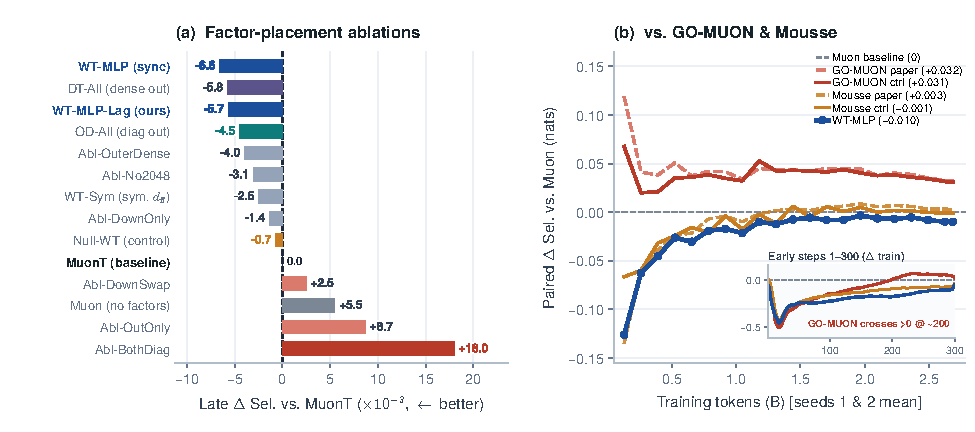
\includegraphics[width=\textwidth]{fig7_ablations_and_related.pdf}
  \caption{\textbf{Design-space ablations and multi-seed comparison against recent polar preconditioners.}
  Unlike \Cref{tab:main_scaling}, differences here are reported against same-wave \mname{MuonT}: these arms vary only the output-side operator at a fixed dense input side, so \mname{MuonT} is the controlled reference. For reference, \mname{MuonT} itself is $-0.0119$ nats below \mname{Muon} in this regime.
  \textbf{(a)} Late-half $\Delta\Lsel$ vs.\ \mname{MuonT} across 14 controlled configurations at \texttt{130M} ($2.68\text{B}$ tokens), showing that dropping input whitening (\mname{Abl-OutOnly}, \mname{Abl-BothDiag}) degrades loss, whereas width-thresholded \mname{WT-MLP} and \mname{WT-MLP-Lag} match or exceed full dense \mname{DT-All}.
  \textbf{(b)} Paired held-out $\Delta\Lsel$ vs.\ \mname{Muon} (mean across fresh \texttt{seeds 1 \& 2}, isotropic matrix decay, $\eta = 0.032$). Inset shows 9-step smoothed early training loss deltas ($\text{steps } 1\text{--}300$): \mname{GO-MUON} plunges $-0.57$ nats by step $18$ before crossing above \mname{Muon} around step $200$ and finishing $+0.031\text{--}0.032$ nats worse, while \mname{Mousse} tracks \mname{Muon} ($\pm 0.003$) and \mname{WT-MLP} maintains a steady $-0.010$-nat lead.}
  \label{fig:ablations_related}
\end{figure}

\subsection{Comparison with Curvature-Aware Polar Baselines (\mname{GO-MUON} and \mname{Mousse})}
\label{sec:related_baselines}

We next benchmark width-thresholded preconditioning against the two closest two-sided polar preconditioners in recent literature:
\mname{GO-MUON}~\citep{che2026gomuon}, which forms activation and observed-cotangent moments with Oracle Approximating Shrinkage (OAS), applies symmetric inverse \emph{quarter} powers $P_B = B^{-1/4}, P_A = C^{-1/4}$ both inside and outside polar orthogonalization, and grafts the result to Frobenius norm $\sqrt{\min(m,n)}$; and
\mname{Mousse}~\citep{zhang2026mousse}, which avoids activation/cotangent hooks by maintaining Shampoo-style weight-gradient Gram EMAs ($G G^{\Tr}, G^{\Tr} G$) with symmetric $-1/8$ powers in eigen-coordinates and post-NS norm grafting.

To separate mathematical geometry from implementation details, we evaluate \emph{both} a controlled profile (sharing our runner's EMA $\beta=0.938$, ridge, refresh cadence, and $\Nten$) and a paper-adapter profile (\mname{GO-MUON}'s OAS shrinkage, compact-SVD polar, and $\beta_B=0.97$ sparse backward EMA; \mname{Mousse}'s pinned 5-stage BF16 polynomial and $\sqrt{m/n}$ scaling), alongside same-runner \mname{Muon} and \mname{WT-MLP} under uniform isotropic matrix weight decay ($\lambda = 0.1$).
After screening all 6 arms across 3 learning rates ($18$ seed-0 runs; every arm selected $\eta = 0.032$), we ran $12$ full-budget ($5{,}120$-step, $2.68\text{B}$-token) confirmations across fresh \texttt{seeds 1 and 2} (\Cref{tab:related}, \Cref{fig:ablations_related}b).

\begin{table}[t]
  \centering
  \caption{\textbf{Controlled multi-seed comparison against \mname{GO-MUON} and \mname{Mousse}} at \texttt{130M} ($2.68\text{B}$ tokens, $5{,}120$ steps, isotropic matrix weight decay $\lambda=0.1$, short-screened $\eta=0.032$, mean across fresh \texttt{seeds 1 \& 2}; standalone synchronous reference harness where ``Total $\Delta t$'' reflects full $5{,}120$-step end-to-end wall-clock time including evaluations).}
  \label{tab:related}
  \vspace{2pt}
  \resizebox{\textwidth}{!}{%
  \begin{tabular}{@{}llrrrrrr@{}}
    \toprule
    Method & Moment Source \& Power Split & Final $\Lsel$ & $\Delta\Lsel$ vs.\ \mname{Muon} & Late $\Delta\Lsel$ & Final $\Lc$ & Step (s) & Total $\Delta t$ \\
    \midrule
    \mname{Muon} (control)  & None; $\Nten(U_t)$                       & $3.2074$ & $0.0000$  & $0.0000$  & $3.4841$ & $1.153$ & $0.0\%$ \\
    \mname{Mousse} (paper)  & Grad Grams $G G^{\Tr}, G^{\Tr}G$; $(-1/8,-1/8)$ & $3.2102$ & $+0.0028$ & $+0.0049$ & $3.4873$ & $1.125$ & $+9.8\%$ \\
    \mname{Mousse} (ctrl)   & Grad Grams $G G^{\Tr}, G^{\Tr}G$; $(-1/8,-1/8)$ & $3.2064$ & $-0.0010$ & $+0.0012$ & $3.4822$ & $1.202$ & $+32.7\%$ \\
    \mname{GO-MUON} (ctrl)  & $C_t, B_t$; $(-1/4,-1/4)$ + norm graft   & $3.2384$ & $+0.0310$ & $+0.0382$ & $3.5135$ & $1.588$ & $+52.0\%$ \\
    \mname{GO-MUON} (paper) & OAS $C_t, B_t$; SVD polar + norm graft   & $3.2395$ & $+0.0321$ & $+0.0397$ & $3.5146$ & $2.021$ & $+94.3\%$ \\
    \rowcolor{rowtint}
    \textcolor{colWT}{\mname{WT-MLP}} & $C_t, B_t$ ($\dff$ diag); $(-1/2,-1/8)$ unit-RMS & \textbf{3.1975} & \textbf{$-$0.0099} & \textbf{$-$0.0071} & \textbf{3.4742} & $1.365$ & $+21.1\%$ \\
    \bottomrule
  \end{tabular}%
  }
\end{table}

Two sharp lessons stand out in \Cref{tab:related} and \Cref{fig:ablations_related}b:
\begin{itemize}[leftmargin=1.5em, itemsep=2pt, topsep=2pt]
  \item \textbf{Why \mname{GO-MUON} dives early then inverts:} During the first $20$ updates, both \mname{GO-MUON} profiles plunge $-0.50$ to $-0.64$ nats below \mname{Muon} (\Cref{fig:ablations_related}b inset), explaining their strong appeal on short-horizon tasks. However, both cross \emph{above} \mname{Muon} around step $180\text{--}210$ and finish $+0.0310$ and $+0.0321$ nats worse at $2.68\text{B}$ tokens ($+52\%\text{--}94\%$ slower). Applying a steep $-1/4$ power \emph{outside} polar orthogonalization coupled with forced $\sqrt{\min(m,n)}$ Frobenius norm grafting over-amplifies noisy cotangent directions once initial transient curvature subsides---validating \mname{MuonT} and \mname{WT-MLP}'s decoupled $(-1/2 \text{ inner},\,-1/8 \text{ outer})$ exponent split.
  \item \textbf{Decoupled moments beat entangled gradient Grams:} \mname{Mousse} finishes within $-0.0010$ (controlled) and $+0.0028$ (paper) of \mname{Muon}, whereas \mname{WT-MLP} outperforms \mname{Muon} by $-0.0099$ nats ($-0.0089$ over \mname{Mousse-Ctrl} on both seeds; also showing that \mname{WT-MLP} retains strong gains under isotropic weight decay). Because $G = \sum_j \delta_j x_j^{\Tr}$, gradient Grams $G G^{\Tr}$ entangle output cotangents with squared activation norms $\|x_j\|_2^2$ and cross-sample interference, losing the clean Kronecker separation of $C_t$ and $B_t$.
\end{itemize}

\subsection{Mechanistic Verification: Subspace Rotation vs.\ Step-Size Scaling}
\label{sec:mechanism}

Recent critiques of spectral optimizers (\citealt{shumaylov2026freon}; \citealt{goyal2026spectrally}) show that apparent geometric gains can stem covertly from altering the effective step-size norm $\|D_t\|_F / \|W_t\|_F$.
To test this hypothesis directly, we perform a counterfactual direction-grafting audit on saved mid-training (step $2{,}500$) and final (step $5{,}120$) checkpoints: holding \mname{MuonT}'s exact weights $W_t$, Nesterov source $U_t$, and right factors $(R_t, \hat{R}_t)$ fixed, we compute the counterfactual update $D_{\text{cand}}$ under \mname{WT-MLP}, \mname{OD-All}, and \mname{DT-All} and compare its Frobenius norm and angle $\theta(D_{\text{cand}}, D_{\text{MuonT}}) = \arccos\frac{\langle D_{\text{cand}}, D_{\text{MuonT}}\rangle}{\|D_{\text{cand}}\|_F \|D_{\text{MuonT}}\|_F}$ across all $224$ matrices (\Cref{fig:mech_pareto}a):

\begin{itemize}[leftmargin=1.5em, itemsep=2pt, topsep=2pt]
  \item \textbf{Zero step-size inflation:} \mname{WT-MLP}'s unit-RMS outer factors slightly \emph{reduce} update Frobenius norm relative to \mname{MuonT} ($\|D_{\text{WT}}\|_F / \|D_{\text{MuonT}}\|_F = 0.9854$, or $-1.46\%$ at step $2{,}500$ and $-1.91\%$ at step $5{,}120$; realized block weight norms are $-2.45\%$ to $-3.00\%$ smaller, vs.\ $-0.11\%$ for \mname{Null-WT}), while rotating update directions by a mean angle of $22.4^\circ$ ($\cos = 0.9218$, nearly matching full dense \mname{DT-All}'s $22.8^\circ$).
  \item \textbf{Mechanistic explanation for \mname{OD-All} falling back onto \mname{MuonT} at \texttt{520M}:} Inspecting rotation angles projection-by-projection (\Cref{fig:mech_pareto}a) reveals that on \texttt{gate} and \texttt{up}, \mname{OD-All} and \mname{WT-MLP} induce nearly identical rotations ($\sim 23^\circ\text{--}26^\circ$; counterfactual $\cos(D_{\text{diag}}, D_{\text{dense}}) = 0.988$ and $0.972$ median). On residual-stream writers \texttt{o} and \texttt{down}, however, \mname{OD-All} rotates \mname{MuonT}'s update by only $4.3^\circ$ and $5.4^\circ$, whereas \mname{WT-MLP} rotates them by $17.7^\circ$ and $17.0^\circ$! Thus \mname{OD-All} leaves residual-stream updates nearly unpreconditioned on the left---a deficit that becomes decisive at width $d = 1{,}024$.
\end{itemize}

\begin{figure}[t]
  \centering
  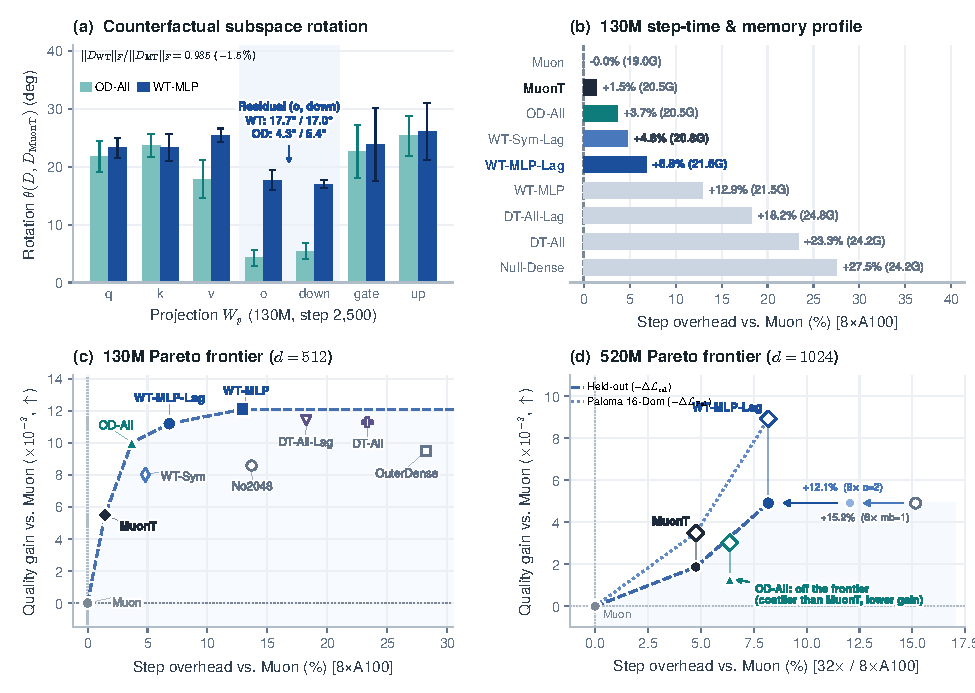
\includegraphics[width=\textwidth]{fig8_mechanism_and_pareto.pdf}
  \caption{\textbf{Mechanistic verification and multi-scale (\texttt{130M} \& \texttt{520M}) quality--overhead Pareto frontiers.}
  \textbf{(a)} Counterfactual update rotation angle $\theta(D, D_{\text{MuonT}})$ at step $2{,}500$ holding $W_t, U_t, R_t, \hat{R}_t$ fixed: \mname{WT-MLP} leaves Frobenius step norm slightly smaller ($0.985\times$) while rotating residual writers \texttt{o} and \texttt{down} by $17.7^\circ$ and $17.0^\circ$ vs.\ \mname{OD-All}'s $4.3^\circ$ and $5.4^\circ$.
  \textbf{(b)} Matched mid-training $8\times\text{A100}$ step-time overhead against \mname{Muon} and peak allocated memory at \texttt{130M} (\texttt{bench\_8gpu\_opt}); input-only \mname{MuonT} already costs $+1.5\%$.
  \textbf{(c)} Design-space Pareto frontier at \texttt{130M} ($d=512$, $8\times\text{A100}$), both axes measured against \mname{Muon}: \mname{WT-MLP-Lag} ($+6.8\%$ step time, $+11.2 \times 10^{-3}$ quality) sits on the sharp knee, strictly dominating dense (\mname{DT-All}, \mname{DT-All-Lag}) and partial (\mname{No2048}, \mname{OuterDense}) variants.
  \textbf{(d)} Width-scaled Pareto frontier at \texttt{520M} ($d=1{,}024$, $10.74\text{B}$ tokens), also against \mname{Muon}: \mname{WT-MLP-Lag} reaches $+4.95 \times 10^{-3}$ late $\Lsel$ and $+8.93 \times 10^{-3}$ 16-domain Paloma for $+8.2\%$ step time, against \mname{MuonT}'s $+1.86$ and $+3.49$ for $+4.8\%$, while pure-diagonal \mname{OD-All} sits below the frontier (gaining less than \mname{MuonT} at higher cost). Arrows trace the systems progression at fixed quality: $+15.2\%$ unchunked on $8\times\text{A100}$, $+12.1\%$ chunked, $+8.2\%$ on $32\times\text{A100}$.}
  \label{fig:mech_pareto}
\end{figure}

\subsection{Unified Multi-Scale Systems Profile and the Compute--Quality Frontier}
\label{sec:pareto}

Finally, to compare systems cost free of cross-node variance, we benchmarked all 19 taxonomic methods from an identical mid-training checkpoint at \texttt{130M} (step $2{,}500$, measuring $60$ post-warmup updates $37\text{--}96$ on $8\times\text{A100}$) alongside matched \texttt{520M} scaling benchmarks across $8\times\text{A100}$ and $32\times\text{A100}$ (full tables in \Cref{app:appendix_systems}).
\Cref{fig:mech_pareto}b--d trace how algorithm--systems co-design reshapes the efficiency frontier across model scales:
\begin{itemize}[leftmargin=1.5em, itemsep=2pt, topsep=2pt]
  \item \textbf{Compressing two-sided overhead by $5\times$:} Naive dense capture/updates (\mname{Null-Dense} $+25.7\%$, \mname{DT-All} $+21.6\%$, $24.2\text{ GiB}$) are strictly dominated. Width thresholding cuts memory by $2.6\text{ GiB}$ ($21.6\text{ GiB}$), and adding $\tau=1$ asynchronous overlap with non-blocking batched fallbacks drops unified benchmark step overhead from $+11.3\%$ (\mname{WT-MLP}) to $+5.29\%$ (\mname{WT-MLP-Lag}) and $+3.32\%$ (\mname{WT-Sym-Lag}).
  \item \textbf{Honest token-budget vs.\ wall-clock trade-off:} At fixed token or data budgets---and in inference-amortized regimes where a pretrained \texttt{130M} or \texttt{520M} model is deployed at scale so final quality per parameter dominates training cost---\mname{WT-MLP-Lag} is a clear winner across every scale and benchmark, reaching $\Lc \le 3.52$ in $5.26\%$ fewer tokens than \mname{MuonT} ($2.36\text{B}$ vs.\ $2.49\text{B}$).
  Measured by pure training wall-clock time to a fixed loss threshold on $8\times\text{A100}$, \mname{WT-MLP-Lag}'s $+5.29\%$ steady-state step-time overhead essentially offsets its $5.26\%$ token saving ($5{,}198\text{ s}$ vs.\ \mname{MuonT}'s $5{,}211\text{ s}$ to $\Lc \le 3.52$ at benchmark median step times, $0.998\times$; $5{,}376\text{ s}$ vs.\ $5{,}212\text{ s}$ under window-mean step times), while \mname{WT-Sym-Lag} reaches the threshold slightly faster ($5{,}100\text{ s}$, $0.979\times$).
  \item \textbf{Proportional overhead scaling to \texttt{520M} across $8\text{--}32\times\text{A100}$:} In our initial unchunked single-node \texttt{520M} run ($8\times\text{A100}$, $\text{microbatch } 1, \texttt{chunk}=0$), $32$-microbatch row-buffer memory pressure ($31.6\text{ GiB}$) and per-matrix fallback syncs raised step overhead to $+15.2\%$ over \mname{Muon} ($5.886\text{ s}$ vs.\ $5.112\text{ s}$; $+10.5\%$ against \mname{MuonT}'s $5.328\text{ s}$). Enabling chunked row-buffer accumulation ($\texttt{chunk}=2$, unlocking $\text{microbatch } 2$ at $30.7\text{ GiB}$) and non-blocking single-call batched \texttt{eigh} fallbacks accelerates all four methods by $8\text{--}12\%$ on a single $8\times\text{A100}$ node ($4.642\text{ s}$ \mname{Muon}, $4.882\text{ s}$ \mname{MuonT}, $4.986\text{ s}$ \mname{OD-All} [$+2.1\%$], and $5.202\text{ s}$ \mname{WT-MLP-Lag} [$+6.6\%$ steady-state; $5.322\text{ s}$ full window---faster than unchunked \mname{MuonT}]). Scaling across $4\times 8 = 32\text{ A100}$ GPUs over RoCEv2 RDMA---which restores \texttt{130M}'s $4$-microbatch accumulation window and $1$-layer-per-rank sharding ($30.7\text{ ms}$ input root time vs.\ $117.4\text{ ms}$ on $8$ GPUs)---reduces step times to $1.322\text{ s}$ (\mname{Muon}), $1.385\text{ s}$ (\mname{MuonT}), $1.406\text{ s}$ (\mname{OD-All}, $+1.5\%$), and $1.431\text{ s}$ (\mname{WT-MLP-Lag}, $+3.3\%$ matched-checkpoint; $1.458\text{ s}$ / $+5.6\%$ from independent warm states, $27.9\text{ GiB}$), confirming that width-thresholded two-sided overhead remains bounded at $\sim 3\text{--}6\%$ as model width scales (\Cref{fig:mech_pareto}d, \Cref{tab:bench520m}).
\end{itemize}
